\subsection{Disk Fitter (tutorial 5)}

Shows a dialog that enables the user to fit an ellipse to a disk. See the usage via \code{python3 ./run_disk_fit.py -h}. An explanation of the interface is given in \figref{fig:disk_fitter}. The code that runs the GUI is in \code{.../scripts/fitscube/fit_disk.py}, and ellipse calculations are in \code{.../scripts/fitscube/geometry/ellipse.py}. Requres the `astroquery' package to run properly. Use \code{pip3 install astroquery}, if there is already a version, ensure you have the newest version by running \code{pip3 install --upgrade astroquery}.

\begin{figure}[h!]
	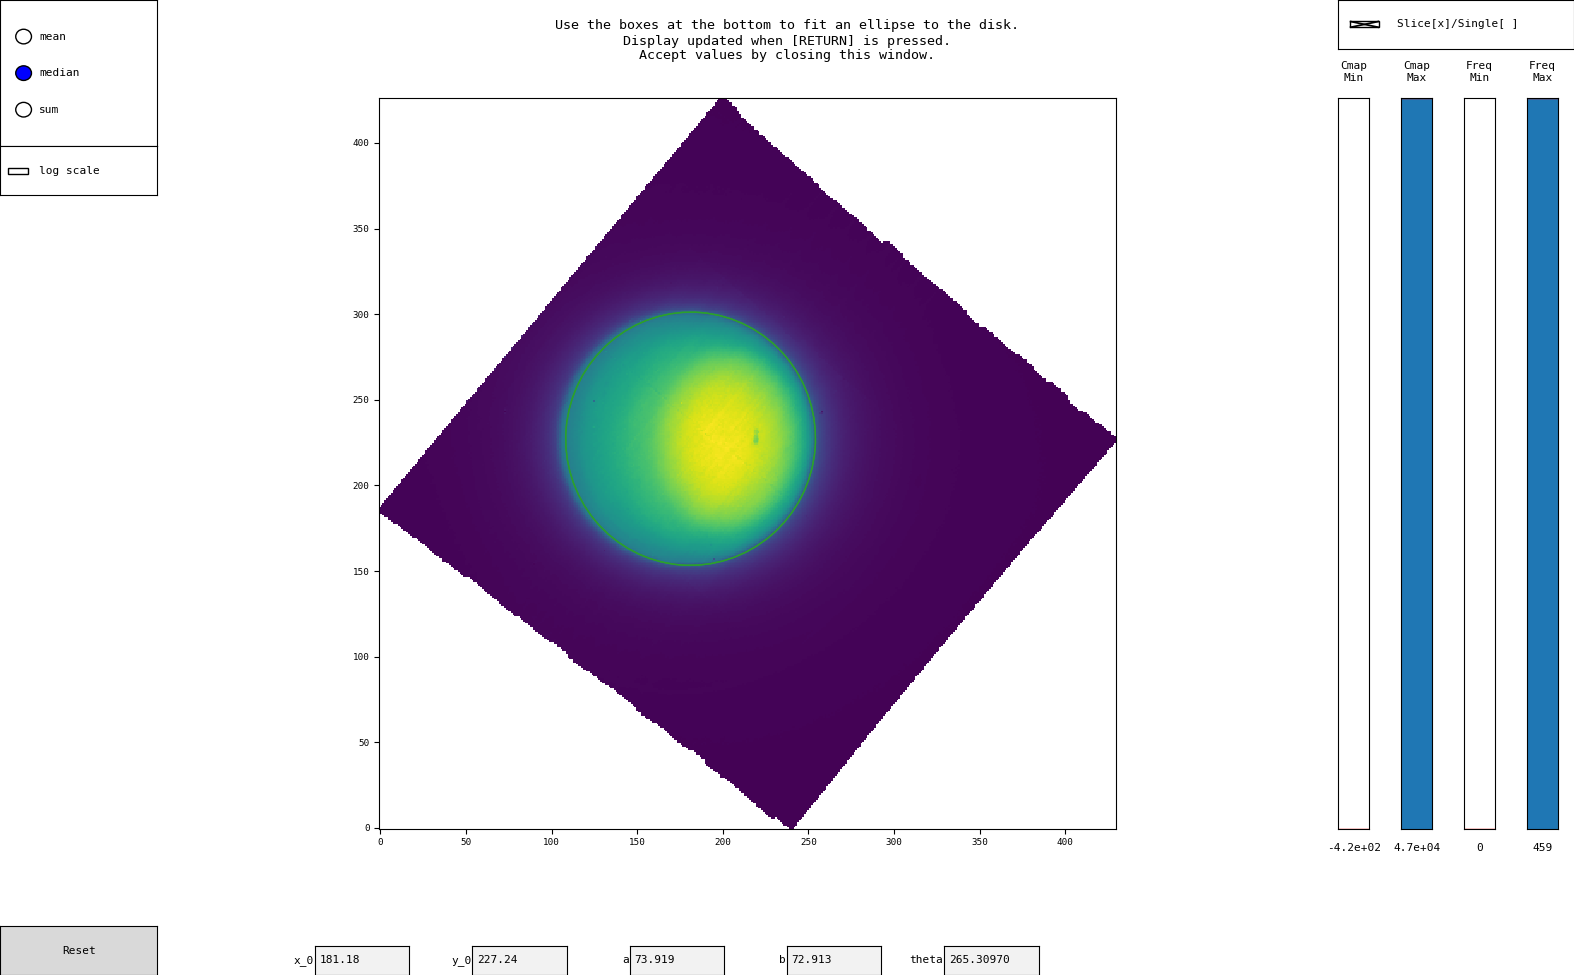
\includegraphics[width=\textwidth]{figures/fitscube_disk_finder.png}
	\caption{\textbf{Main Center Panel:} Shows the datacube with an ellipse (green, hard to see here) superimposed upon it. \textbf{Top Right:} Changes between multi and single channel mode, in multi-channel mode the image is a combination of all channels in the range as set by the selector in the top left. \textbf{Middle Right:} Colour map limits (Cmap Min, Cmap Max) and frequency channel limits (Freq Min, Freq Max). Clicking will set the relevant bar, values are shown at the bottom of the bars. Single-channel mode only shows a single frequency selector. \textbf{Top Left:} Aggregate selector swaps between combining channels via mean, median, or sum in multi-channel mode (unused in single-channel mode). Logarithmic scale can be toggled on or off. \textbf{Bottom Row:} `Reset' button resets all controls to their defaults. `x{\textunderscore}0' moves the ellipse center in the x-direction, `y{\textunderscore}0' moves the ellipse center in the y-direction. `a' changes the semi-major axis of the ellipse. `b' changes the semi-minor axis of the ellipse. `theta' rotates the ellipse. All numbers are given in pixels, fractions are possible. Close the dialog to accept the current values and continue with calculation.}
\label{fig:disk_fitter}
\end{figure}



\subsection{Webservices}

Located in \code{.../scripts/webservices}, there are two python files. \code{jplhorizons.py} has a couple of helper-functions based on `astroquery' to get ephemeris data from JPL-Horizons. \code{observatory_codes.py} holds routines that grab observatory codes from the internet and associate them with their names.


\subsection{Nemesis}

Located in \code{.../scripts/nemesis} most of these routines are superceeded by \textsc{nemesispy}. However, some of them may be useful and other scripts that interface with nemesis require them.


\subsection{fitscube/process}

Contains processing scripts for \textsc{sinfoni} data. Most of it is old and obsolete.

\subsection{astro{\textunderscore}resources.py}

\code{../scripts/astro_resources.py} contains some data about the physical parameters of planets. Used by the disk-fitting routines to get the sizes correct.